\selectlanguage{english}
\begin{abstract}
    \noindent For the first project of the Computer Simulations (ELTE Physics MSc) course I propose a concept of an N-body simulation, which aims to reproduce the satellite formation inside asteroid belts around a larger stellar object (eg. a gas giant or a star). Due to the N-body simulations' high computational difficulty, my spare objective is to observe at least some form of clustering process inside these type of systems. To achieve these goals, I will use Newton's law of universal gravitation, solving the particles' equation of motion by a simple 4th order Runge-Kutta function. Other numerical methods - described in Sec. III. will be optionally tested.
\end{abstract}

\begin{multicols}{2}
\section{Introduction}
The problem of gravitational- or electromagnetic attraction of more, than 2 bodies are impossible to solve analitically, except for some finite special cases. To study the motion of the particles in such systems we're ought to rely on numerical simulations and approximations. The computational difficulty of the problem grows non-linearly as we try to simulate more and more particles, and thus these simulations are required to be reinforced by some clever numerical tricks to overcome the barrier of immense computational times. \par
In this project I tried to create a gravitational n-body simulation, which could be used to simulate the motion of relatively small, but still interesting amount of bodies. As I've achieved pretty good values for runtime, it was still too slow, to simulate a system with eg. 1000 bodies on my personal computer for hundreds of years. In this paper I present my current results at the deadline.

\section{Theoretical background}
In the short description I've already covered some of the theoretical background of the gravitational n-body problem. I've already wrote, that the force, acting on the $i$th body could be described by the following sum:

\begin{equation} \label{eq:1}
m_{i} \boldsymbol{\ddot{r}}_{i}
=
- G \sum_{i \neq j} \frac{m_{i} m_{j}}{\left| r_{i} - r_{j} \right|^{2}} \frac{\boldsymbol{r}_{i} - \boldsymbol{r}_{j}}{\left| r_{i} - r_{j} \right|}
\end{equation}
Using this, one can simply describe the acceleration acting on the $i$th body:

\begin{equation} \label{eq:2}
\boldsymbol{\ddot{r}}_{i}
=
- G \sum_{i \neq j} \frac{m_{j}}{\left| r_{i} - r_{j} \right|^{2}} \frac{\boldsymbol{r}_{i} - \boldsymbol{r}_{j}}{\left| r_{i} - r_{j} \right|}
\end{equation}
Which differential equation essentially should be solved numerically for the $x$, $y$ and $z$ components of the $\boldsymbol{r}$ vector to acquire the coordinates and velocities of the individual particles. \par
In 3D coordinates it is an article-level problem to study the possible 3D trajectories \citep{3Dtrajectory} and the system could be seriously unstable. After acknowledging these facts, I decided to study the behavior of the setup, where the objects are scattered in a 2D plane around a central object. In my simulations the central object was the Jupiter, and the objects around it symbolized the asteroid belt.

\section{Preliminary setup of the simulation}
To unambiguously define the initial setup of the system, I decided to create an asteroid-generation pipeline, following the same steps in order in the generation of every new objects. \par
At the I. step the size and mass of the central object where chosen, along with number of small bodies as well. \par
At the II. step the pipeline generated spherical bodies with various sizes, but constant densities. The masses were calculated next from these two values. Here, only the minimal and maximal radius of the small bodies were given to the pipeline. For the densities I've chosen $\rho_{S} = 2270\ \text{kg}/\text{m}^{3}$ consistently, which is a relatively medium-size value for asteroids \citep{krasinsky2002hidden}. \par
At the III. step the initial coordinates and velocities of the small bodies were generated. According to Kepler's first law, a satellite orbits a central object on an elliptic orbit, where the central object is situated in one of the focal points. When the object is gravitationally bound, its orbit's shape is an ellipse or in special case, a circle. The distance of the satellite from the central body could be easily expressed:

\begin{equation} \label{eq:3}
d
=
\frac{r_{p}}{1 + e * \cos{\varphi}}
\end{equation}
where $r_{p}$ is the length of the perigee, $e$ is the eccentricity, $\varphi$ is the polar angle. Here, I generated random $r_{p}$ perigee distances and $e$ eccentricities from a pre-defined interval. The possible perigee distances' values were $r_{p} = 10 R \pm 1.5 R$, where $R$ is the radius of the central planet, while the maximal eccentricity was chosen to be $e_{max} = 0.4$. Using this two values, the semi-major ($a$) and semi-minor ($b$) axis of the trajectories for every body could be calculated, as follows:

\begin{equation} \label{eq:4}
a = \frac{r_{p}}{1 - e^2}
\end{equation}
\begin{equation} \label{eq:5}
b = \frac{r_{p}}{\sqrt{1 - e^2}}
\end{equation}
After this, I generated a random $\varphi$ azimuth angle and calculated the coordinates, using the following forms:

\begin{equation} \label{eq:6}
\begin{pmatrix}
x \\
y
\end{pmatrix}
=
\begin{pmatrix}
a * \cos{\varphi} \\
b * \sin{\varphi}
\end{pmatrix}
\end{equation}
Using the Vis-Viva equation the length of the velocity vector $\left| \boldsymbol{v} \right|$ could be calculated, if the initial setup for every small body is considered as a two-body problem of the asteroid and the central object. Since the masses of the small bodies are very small, compared the to central object, it is a perfectly fine to use this approximation.

\begin{equation} \label{eq:7}
\left| \boldsymbol{v} \right|
=
\sqrt{GM \left( \frac{2}{a} - \frac{1}{d} \right)}
\end{equation}
where $G$ is the gravitational constant, $M$ is the mass of the central object, $a$ is the semi-major axis of the currently described small body, $d$ is the distance of this body from the central object's center of mass. We also know, that the velocity vector always a tangent of the satellites trajectory in every point. It could be calculated by taking the gradient of the ellipse's coordinates:

\begin{equation} \label{eq:8}
\boldsymbol{e}_{t}
=
\frac{\boldsymbol{\nabla} \boldsymbol{r}}{\left| \boldsymbol{\nabla} \boldsymbol{r} \right|}
=
\frac{1}{\left| \boldsymbol{\nabla} \boldsymbol{r} \right|}
\boldsymbol{\nabla}
\begin{pmatrix}
x \\
y
\end{pmatrix}
=
\frac{1}{\left| \boldsymbol{\nabla} \boldsymbol{r} \right|}
\boldsymbol{\nabla}
\begin{pmatrix}
a * \cos{\varphi} \\
b * \sin{\varphi}
\end{pmatrix}
\end{equation}
\begin{equation} \label{eq:9}
\boldsymbol{e}_{t}
=
\frac{1}{\left| \boldsymbol{\nabla} \boldsymbol{r} \right|}
\begin{pmatrix}
-a * \sin{\varphi} \\
b * \cos{\varphi}
\end{pmatrix}
\end{equation}
The actual velocity vector then could be written in the following form, using the result from the (\ref{eq:7}) equation:

\begin{equation} \label{eq:10}
\boldsymbol{v}_{t}
=
\frac{\left| \boldsymbol{v} \right|}{\left| \boldsymbol{\nabla} \boldsymbol{r} \right|}
\begin{pmatrix}
-a * \sin{\varphi} \\
b * \cos{\varphi}
\end{pmatrix}
\end{equation}
After acquiring the velocity vectors and coordinates, the (\ref{eq:2}) differential equation could be solved for every $i$th object numerically.

\section{Technical details}
Since I used Python (especially Jupyter Notebook) for my simulation, it was crucial to speed up the process, since Python is not the fastest programming language regarding runtime. I used two different methods to achieve a speed-up. First, the simulation only calculated the $j$th force acting on the $i$th object, if the asteroids, indexed by $i$ and $j$ were closer, than $2R$ to each other. Second, I used the \texttt{numba} library's \texttt{@jit(nopython=True)} decorator to greatly optimize my code. This decorator compiles the Python functions into machine code before running them, thus greatly enhancing the runtime. Sadly it has strict limitations, so I was forced to write my code accordingly. \par
The full source code, used files and everything related to the project could be found in my GitHub repository of this course\footnote{\url{https://github.com/masterdesky/ELTE\_Comp\_Simulations\_2020}}.

\section{Solving the differential equations}
To solve the equation of motions numerically for all bodies, I used a simple (not adaptive) fourth-order Runge-Kutta function. The functionality of this iterative algorithm is well-known and is the following:

\begin{equation}
k_{1} = dt * \dot{y}_{n}
\end{equation}
\begin{equation}
k_{2} = dt * \left( \dot{y}_{n} + 0.5 * k_1 \right)
\end{equation}
\begin{equation}
k_{3} = dt * \left( \dot{y}_{n} + 0.5 * k_2 \right)
\end{equation}
\begin{equation}
k_{4} = dt * \left( \dot{y}_{n} + k_3 \right)
\end{equation}
\begin{equation}
dy = \frac{k_{1} + 2 * k_{2} + 2 * k_{3} + k_{4}}{6}
\end{equation}
\begin{equation}
y_{n+1} = y_{n} + dy
\end{equation}
In the simulation the $\dot{y}_{n}$ represented the $\dot{r}$ and $\ddot{r}$ values as well, which were incremented by parallel.

\section{Results and problems}
The results were quite disappointing, and I didn't have enough time to fix the trivial, but crucial problem with my simulation. The whole code works very well, at least it doesn't have any logical or physical flaws. The main problem was, that immediately from the beginning, the orbiting bodies' kinetic energy started to grow, which is quite a surprise for an RK4 algorithm, as it is much more common phenomenon, when using the simple Euler's method. \par
After many unsuccessful fixing attempt, - at first glance - I finally solved the problem by choosing the time-step to a smaller value. By trial and error I found, that with $dt \leq 0.001$ years, the simulation becomes highly unstable. Maybe this could be still an acceptable and working parameter, if I'd change RK4 to some higher-order Runge-Kutta function, but I've had very limited time, as I've mentioned it already. Sadly, RK4 still didn't reserved kinetic energy for longer time periods, and started to slightly, but continuously grow. The effect caused by choosing different time steps could be objectively observed by starting the simulation from the same initial conditions with different $dt$ values and let it run for some time.

\begin{center}
    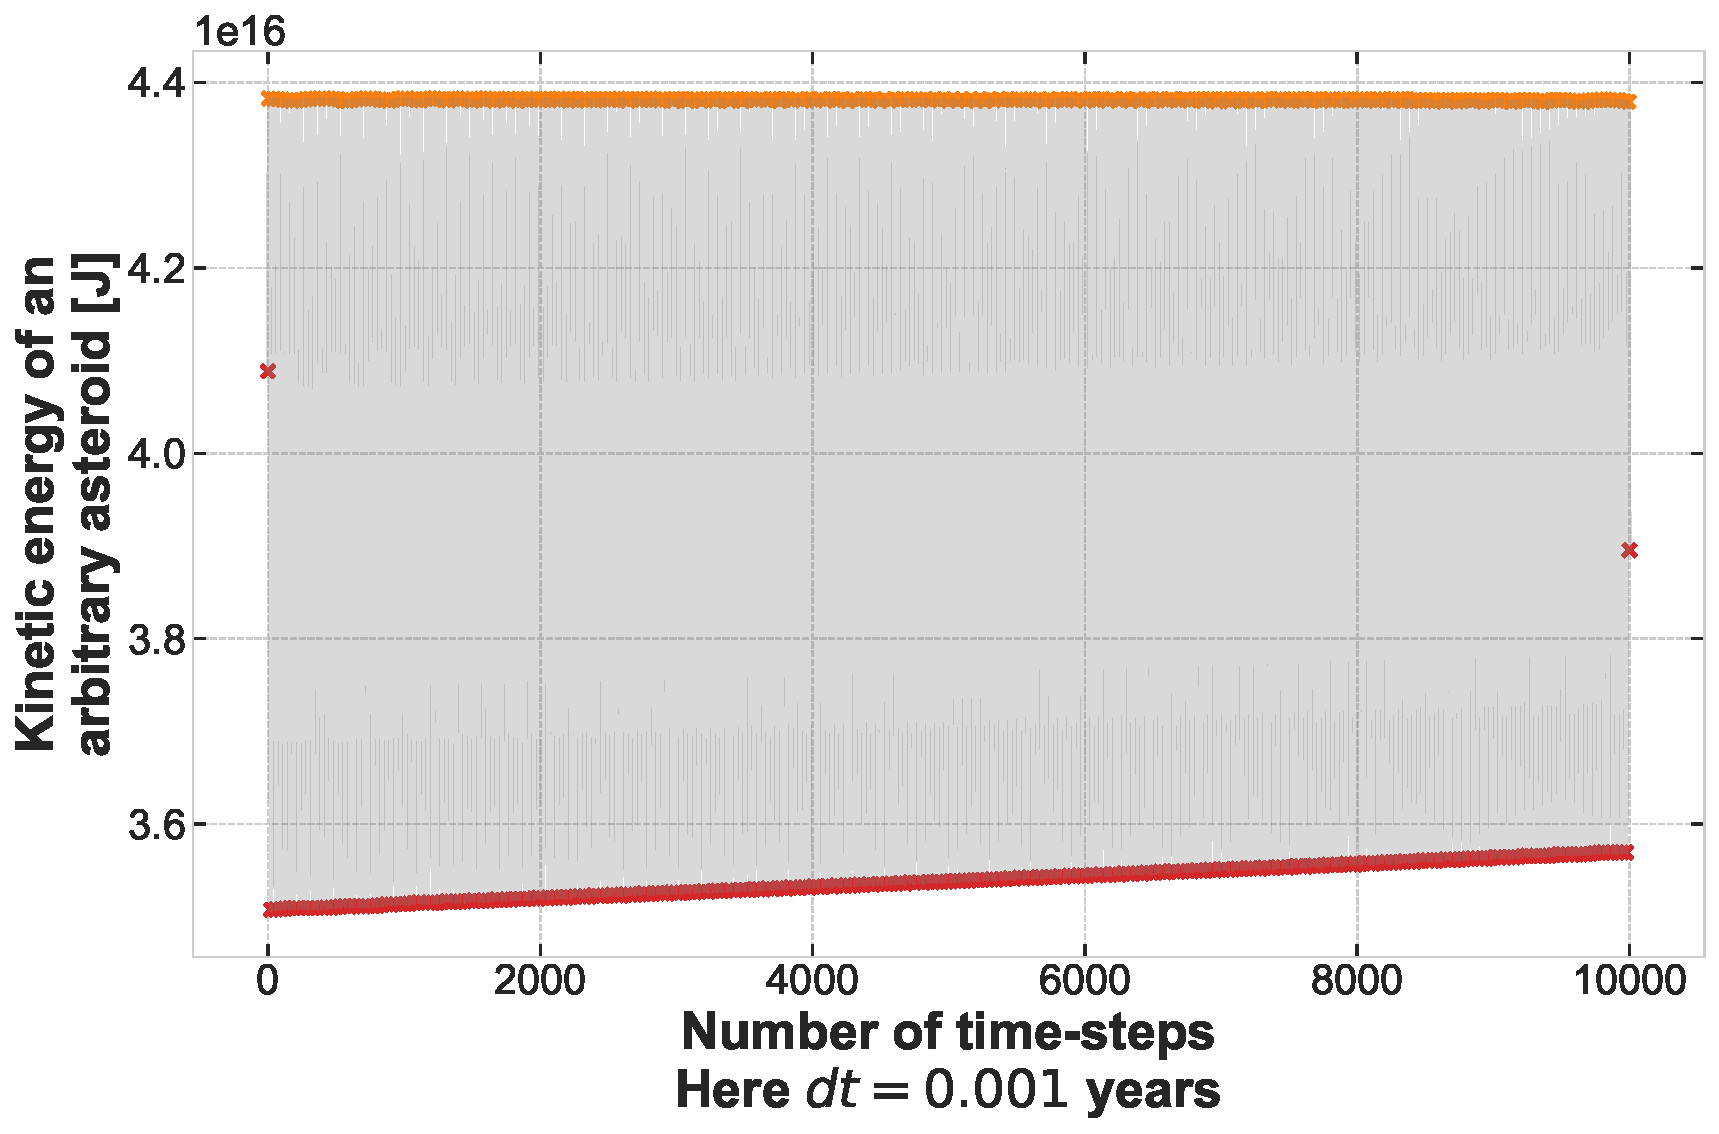
\includegraphics[width=0.5\textwidth]{{img_src/kin_E_max_10_y_dt_0.001_y}.pdf}
    \captionof{figure}{Kinetic energy changes of an arbitrary satellite with time step $dt=0.001$ for $10$ simulated years. A slight grow of the curve could be observed. The local extremas are marked by red and oranges 'X' markers.} \label{fig:1}
\end{center}
Using the time step $dt=0.001$ for $10$ simulated years, the final arrangement of the simulated asteroids could be seen on figure (\ref{fig:4}) and figure (\ref{fig:5}). Running the simulation even further, the energy growth of the small objects in the simulated asteroid belt simply blew up the simulation, as they started to move exponentially faster every iteration after some time.
\begin{center}
    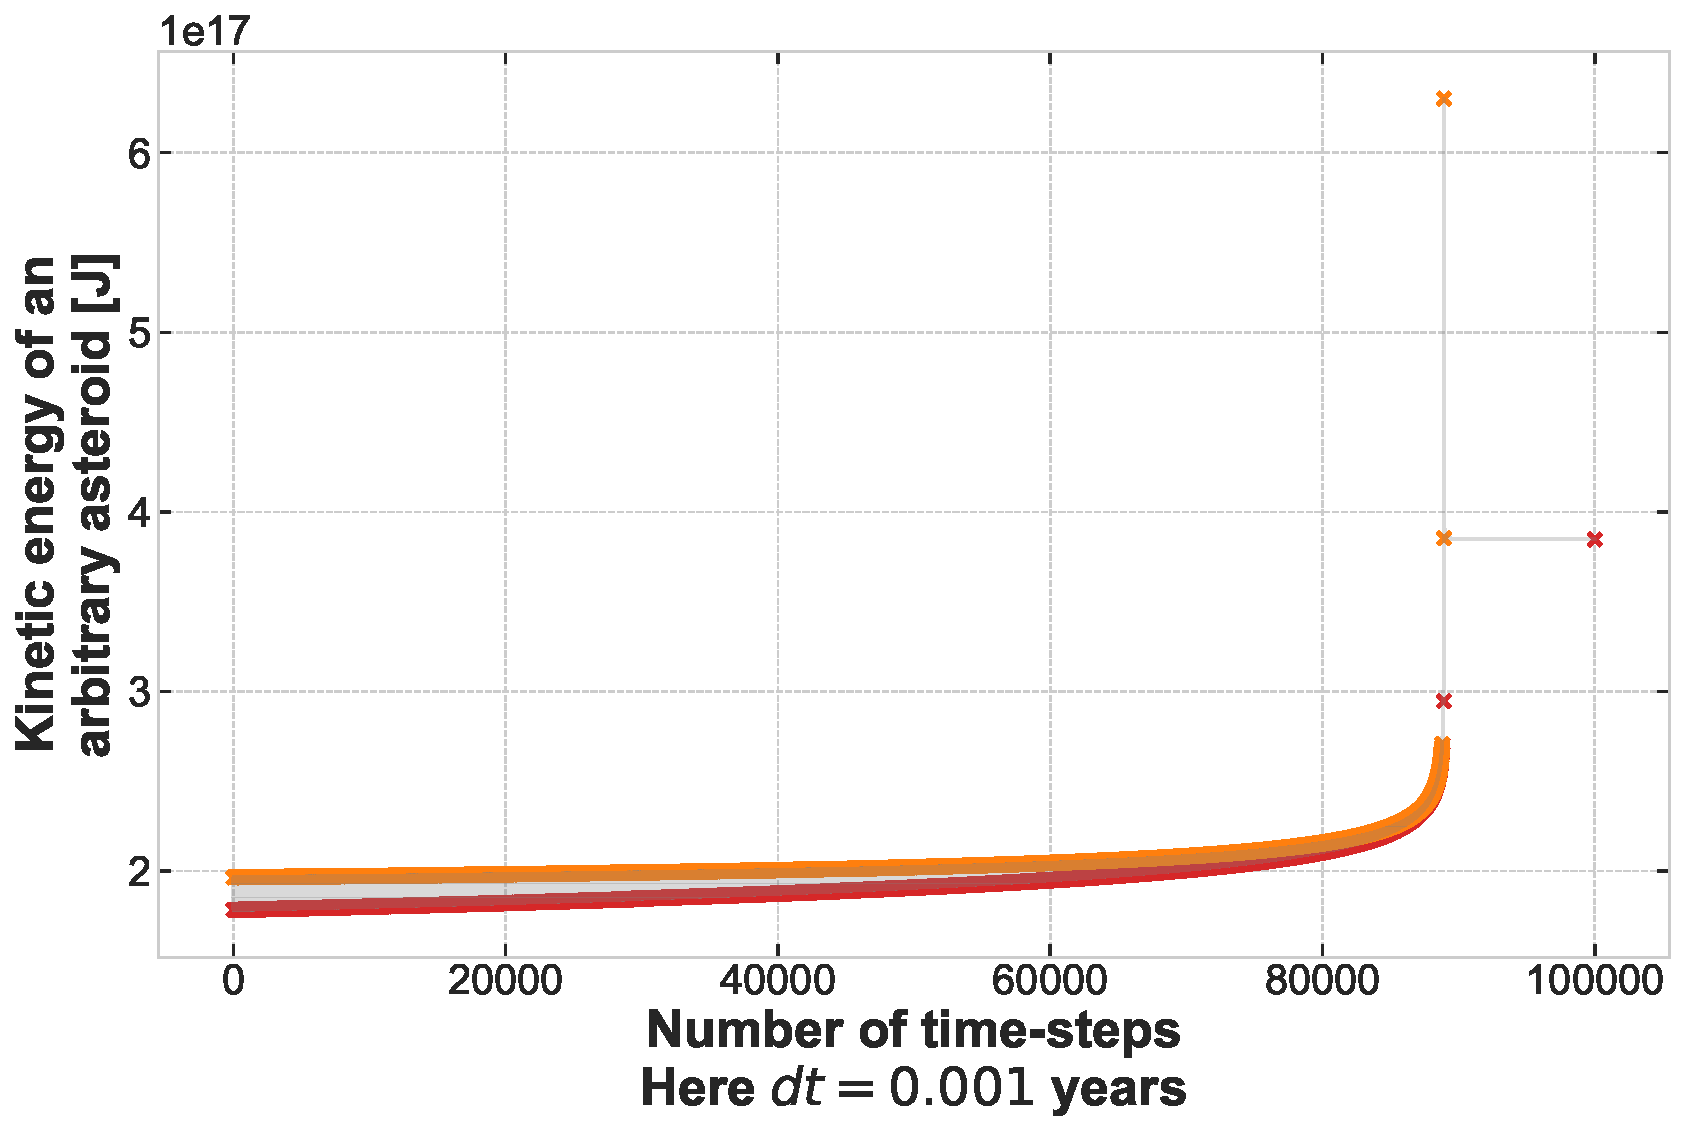
\includegraphics[width=0.5\textwidth]{{img_src/kin_E_max_100_y_dt_0.001_y}.pdf}
    \captionof{figure}{Kinetic energy changes of an arbitrary satellite with time step $dt=0.001$ for $100$ simulated years. A slight grow of the curve could be observed early, then an exponential upstream blows up the simulation. The local extrema are marked by red and oranges 'X' markers. The growth could be seen best by observing the slope of the red line.} \label{fig:2}
\end{center}
In contrast, choosing the step size parameter as $dt = 0.0001$, the energy seemed to remain conserved and the simulation remained totally stable.
\begin{center}
    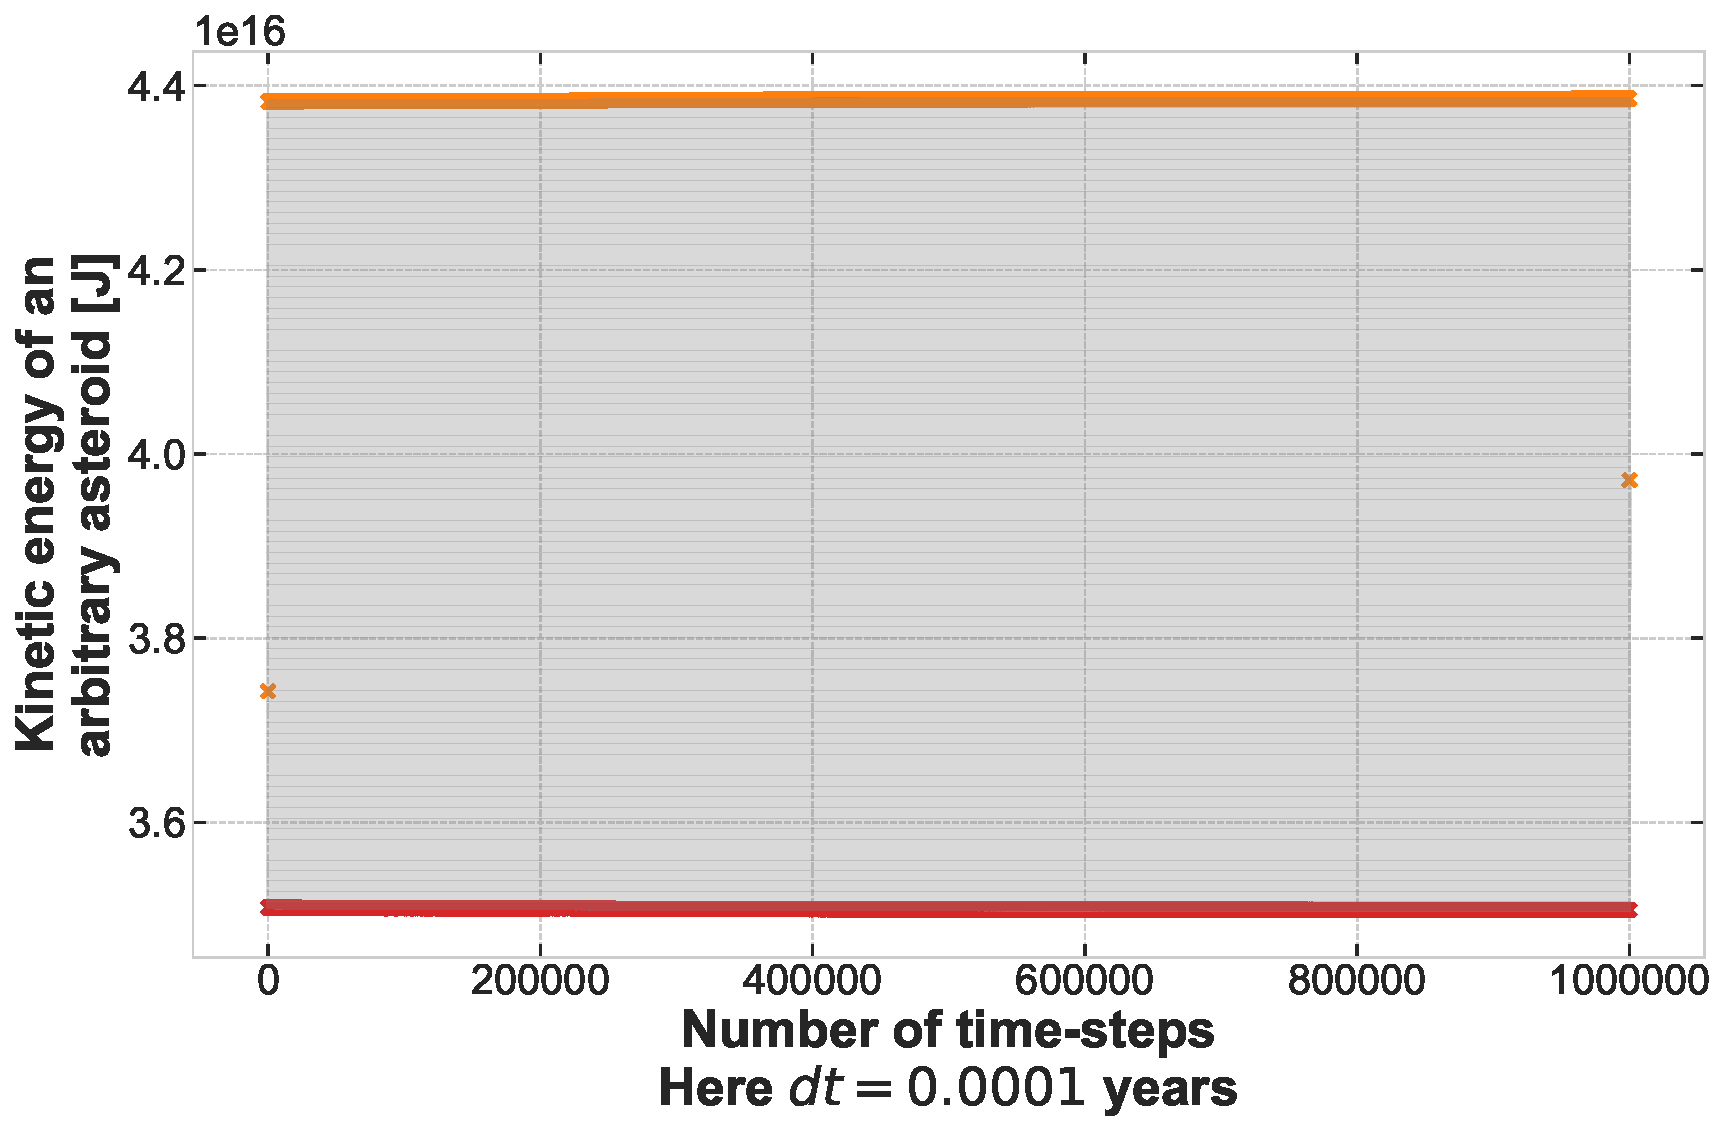
\includegraphics[width=0.5\textwidth]{{img_src/kin_E_max_100_y_dt_0.0001_y}.pdf}
    \captionof{figure}{Kinetic energy changes of an arbitrary satellite with time step $dt=0.0001$ for $100$ simulated years. There are no relevant energy growth could be seen. The local extrema are marked by red and oranges 'X' markers.} \label{fig:3}
\end{center}
The final positions and velocities of the small bodies, running the simulation with these parameters could be seen on Fig. (\ref{fig:6}) and Fig. (\ref{fig:7}). It seems a wise choice to run the simulation with $dt=0.0001$ and let it run for a long time. However it would still not yield any useful results regarding the moon formation or clustering of bodies in an asteroid belt. The total runtime for $100$ years with this time step was $5.25$ hours, but we should simulate at least a few million years to get any kind of results. The simulation maybe could be made "faster", if we would simulate a system, where the asteroids orbit a gas giant, which also orbits a star, thus creating Lagrangian points, where the small bodies could accumulate easier.

\section{Discussion}
At least, I've successfully built a gravitational n-body problem simulation, which could handle time steps relatively fast. Since I couldn't let the simulation run for longer time, and with smaller time steps, I couldn't detect any kind of gravitational clustering, or Moon-formation in an asteroid belt. However I proposed some ideas, which could be further examined in the future. \par
I've also made some animations of the working simulation, which could be reached on my YouTube channel\footnote{\url{https://www.youtube.com/channel/UCBDSB7PdQ3E9l9WSBsTy7cQ}}, under the "Planetary Motions" playlist.

\end{multicols}